\documentclass{article}
\usepackage{amsfonts}
\usepackage{amsmath}
\usepackage{amssymb}
\usepackage{amsthm}
\usepackage{mathtools}
\usepackage{mathrsfs}


% TEXT MARGINS
\setlength{\topmargin}{-0.9in}
\setlength{\textwidth}{6.3in} 
\setlength{\textheight}{9.1in}
\setlength{\oddsidemargin}{-.1in}
\setlength{\parindent}{15pt}
\setlength{\parskip}{2pt}
\parskip 4pt


\usepackage{blkarray}
% \usepackage{caption}
% \DeclareCaptionType{equ}[][]
\usepackage{newtxtext}
\usepackage{verbatim}
\usepackage{placeins}
% \usepackage{nicematrix}
\usepackage[utf8]{inputenc}
\usepackage{tikz}
\usetikzlibrary{shapes.geometric} 
\usetikzlibrary{arrows.meta, bending, positioning, calc} 
\usepackage{graphicx} 
\usepackage[hidelinks]{hyperref}
\usepackage[capitalize]{cleveref}

\usepackage{showlabels}
\usepackage{environ}


\usepackage[pagewise]{lineno}
\usepackage[all]{xy}%for diagrams
\usepackage{array}
\usepackage{comment}
\usepackage[overload]{empheq}



\graphicspath{ {./Figures/} }
\usepackage{placeins, microtype}
\usepackage{latexsym,xcolor,longtable}
\usepackage[notref,notcite]{showkeys}
\DeclarePairedDelimiter\ceil{\lceil}{\rceil}
\DeclarePairedDelimiter\floor{\lfloor}{\rfloor}

\linenumbers






% ENVIRONMENTS

\newenvironment{collapse}{}{}
\newif\ifhideproofs
%\hideproofstrue %uncomment to hide proofs

\ifhideproofs
\NewEnviron{hide}{}
\let\proof\hide
\let\endproof\endhide
\fi


\newtheorem{thm}{Theorem}
\newtheorem{lemma}{Lemma}
\newtheorem{prop}{Proposition}
\newtheorem{corollary}{Corollary}
\newtheorem{conjecture}{Conjecture} 

\theoremstyle{definition}
\newtheorem{definition}{Definition}
\newtheorem{assumption}{Assumption}
\newtheorem{claim}{Claim}
\newtheorem{remark}{Remark}
\newtheorem{example}{Example} 
\newtheorem{question}{Question} 
\newtheorem{exercise}{Exercise} 
\newtheorem{problem}{Problem} 
\newtheorem{algorithm}{Algorithm} 



% SYMBOL ABREVIATIONS
\def\S{\mathcal S}
\def\C{\mathcal C}
\def\Re{\mathcal R}
\def\PP{{\mathcal P}} 
\def\KK{{\mathcal K}} 
\def\A{\boldsymbol{\alpha}}
\def\R{\mathbb{R}}
\def\Z{\mathbb{Z}}
\def\P{{\mathbb P}}     
\def\E{{\mathbb E}} 

%norm
\DeclarePairedDelimiter{\abs}{\lvert}{\rvert}
\DeclarePairedDelimiter{\norm}{\lVert}{\rVert}
\NewDocumentCommand{\supn}{ s O{} m }{%    
  \IfBooleanTF{#1}{\norm*{#3}}{\norm[#2]{#3}}_{\infty}%
}

%bold hat
\newcommand{\thickhat}[1]{\mathbf{\hat{\text{$#1$}}}}


\def\eqd{\,{\buildrel d \over =}\,}
    
\newcommand{\toD}{\,{\buildrel{\rm dist.} \over \longrightarrow}\,}


\newcommand{\equalD}{\,{\buildrel \mathcal{L} \over =}\,}
\newcommand{\bfd}{\boldsymbol{d}}
\newcommand{\Cstar}{\mathcal{C}^*(\mathbb{R}_{+}\times \mathbb{X})}
\newcommand{\clf}{\mathcal{F}}
\newcommand{\clc}{\mathcal{C}}
\newcommand{\clp}{\mathcal{P}}
\newcommand{\clw}{\mathcal{W}}
\newcommand{\clh}{\mathcal{H}}
\newcommand{\rr}{r}
\newcommand{\Err}{\mathcal{R}}
\newcommand{\ind}{\boldsymbol{1}}
\newcommand{\RW}{\textcolor{brown}}
\newcommand{\vt}{\vskip 5mm} % vertical space
\newcommand{\fl}{\noindent\textbf} % first line
\newcommand{\Fl}{\vt\noindent\textbf} % first line with space above
\newcommand{\indep}{\perp \!\!\! \perp}  %independence symbol



\title{Note:  Formalizing combinatorial matrix identities}

\author{} %Dimitris D, @Steven Creech, @Susanna Fishel, @Harry Richman and one more person

\date{ICERM, Apr 24 - 27, 2025} 


\begin{document}

\maketitle

\begin{abstract}

\end{abstract}

\noindent
\textbf{Github repository} It is available here
\begin{center}
    \url{https://github.com/harryrichman/lean-graph-matrices}
\end{center}

\section{April 24th, ICERM}

\subsection{Theoretical background knowledge}


Something with types. . .. 





\subsection{Notation and problem statement}

The Laplacian of a graph $G=(V,E)$ is a matrix associated with a graph. Let $D$ be the degree matrix that keeps track of the degrees of each node of the graph on its diagonal entries. Let $A$ be the adjacency matrix of the graph (add $1$ in the entries for which there is a corresponding edge on the graph). Then
\begin{equation}
    L:=D-A.
\end{equation}

To state the desired theorem we also state the following. First, whenever we remove the row and column associated with the $q$-th entry of a matrix $M$ we write $M\mid q$ $M |_{q}$.

\begin{thm}\label{Thm:main}
    Let $G=(V,E)$ be a simple finite graph, then for any vertex $q \in V$ it holds that
    \begin{equation}
        det(L\mid q)=\#\text{ spanning trees of }G.
    \end{equation}
\end{thm}


\subsection{Resources and background material}



\noindent
\textbf{Search tools} (in human language) that could help  find functions of mathbib that might be relevant to the project please go to the following.
\begin{itemize}
    \item LearnSearch
    \item Moogle
    \item Zulip chat
    \item Loogle
\end{itemize}


\noindent
\textbf{Mathematics preliminaries} For our problem, some key ingredients include the following
\begin{itemize}
    \item Laplacian of a matrix
    \item Spanning tree
    \item Matrix minor
    \item Determinant
    \item Subgraph
    
\end{itemize}

\subsection{Triangles}

A triangle is one of the simplest possible graph, 
\begin{center}
    \begin{tikzpicture}[scale=1.5, every node/.style={circle, draw, minimum size=1cm}]
    % Nodes
    \node (A) at (0, 0) {1};
    \node (B) at (2, 0) {2};
    \node (C) at (1, 1.73) {3}; % height of equilateral triangle with side length 2

    % Edges
    \draw (A) -- (B);
    \draw (B) -- (C);
    \draw (C) -- (A);
\end{tikzpicture}
\end{center}
Then the adjacency matrix is
$$
A = \begin{bmatrix}
0 & 1 & 1 \\
1 & 0 & 1 \\
1 & 1 & 0 \\
\end{bmatrix}
$$
and the degree matrix is 
$$
D = \begin{bmatrix}
2 & 0 & 0 \\
0 & 2 & 0 \\
0 & 0 & 2 \\
\end{bmatrix}
$$
thus the Laplacian matrix is
$$
L = \begin{bmatrix}
2 & -1 & -1 \\
-1 & 2 & -1 \\
-1 & -1 & 2 \\
\end{bmatrix}
$$


\subsection{A less simple example}

Let $G=(V,E)$ be the  graph depicted below
\begin{center}
    \begin{tikzpicture}[scale=0.5, every node/.style={circle, draw, minimum size=0.5cm}]
    % Nodes
    \node (1) at (0,0) {1};
    \node (2) at (2,2) {2};
    \node (3) at (4,0) {3};
    \node (4) at (2,-1.5) {4};
    \node (5) at (2,4) {5};

    % Edges
    \draw (1) -- (4);
    \draw (1) -- (5);
    
    \draw (2) -- (3);
    \draw (2) -- (4);
    \draw (2) -- (5);

    \draw (3) -- (4);

    \draw (4) -- (1); % already drawn, but repeating doesn't hurt
    \draw (5) -- (1); % same

\end{tikzpicture}
\end{center}
then its adjacency matrix is 
$$
A = \begin{bmatrix}
0 & 0 & 0 & 1 & 1 \\
0 & 0 & 1 & 1 & 1 \\
0 & 1 & 0 & 1 & 0 \\
1 & 1 & 1 & 0 & 0 \\
1 & 1 & 0 & 0 & 0 \\
\end{bmatrix}
$$
and degree matrix
$$
D = \begin{bmatrix}
2 & 0 & 0 & 0 & 0 \\
0 & 3 & 0 & 0 & 0 \\
0 & 0 & 2 & 0 & 0 \\
0 & 0 & 0 & 3 & 0 \\
0 & 0 & 0 & 0 & 2 \\
\end{bmatrix}
$$
and thus the Laplacian matrix is 
$$
L = \begin{bmatrix}
2 & 0 & 0 & -1 & -1 \\
0 & 3 & -1 & -1 & -1 \\
0 & -1 & 2 & -1 & 0 \\
-1 & -1 & -1 & 3 & 0 \\
-1 & -1 & 0 & 0 & 2 \\
\end{bmatrix}
$$
\begin{remark}[sanity check]% \rm
    Two tests for checking the validity of a Laplacian matrix associated with a graph is as follows. 
    First, the elements of each row and each column should add up to $0$. 
    Second, the diagonal should have non negative entries.
\end{remark}
Now, according to Theorem~\ref{Thm:main}, the number of spanning tree is equal to 
$$
  det(L\mid 3)=....=29?
$$

 
\end{document}